%%%% Generic manuscript mode, required for submission
%%%% and peer review
\documentclass[manuscript,screen,sigplan]{acmart}
\settopmatter{printfolios=true,printccs=false,printacmref=false,}

%% Rights management information.  This information is sent to you
%% when you complete the rights form.  These commands have SAMPLE
%% values in them; it is your responsibility as an author to replace
%% the commands and values with those provided to you when you
%% complete the rights form.
%%\setcopyright{XXX}
%%\copyrightyear{XXXX}
%%\acmYear{XXXX}
%%\acmDOI{XXXXXXX.XXXXXXX}

%% These commands are for a PROCEEDINGS abstract or paper.
\acmConference[OCaml Workshop '22]{International Conference on Functional Programming}{Sept 11--16,
  2022}{Ljubljana, Slovenia}

\usepackage{listings}
\usepackage{amsthm}
\usepackage{graphicx}
\usepackage{hyperref}
\hypersetup{hidelinks = false}


%% Bibliography style
%%\bibliographystyle{ACM-Reference-Format}
%%\citestyle{acmauthoryear}   %% For author/year citations


\lstset{
  language=caml,
  basicstyle=\ttfamily
}

%%
%% end of the preamble, start of the body of the document source.
\begin{document}

%%
%% The "title" command has an optional parameter,
%% allowing the author to define a "short title" to be used in page headers.
\title{OBuilder - Homogeneous builds with OCaml}

%%
%% The "author" command and its associated commands are used to define
%% the authors and their affiliations.
%% Of note is the shared affiliation of the first two authors, and the
%% "authornote" and "authornotemark" commands
%% used to denote shared contribution to the research.
\author{David Allsopp, Kate Deplaix, Patrick Ferris, Thomas Leonard, Anil Madhavapeddy}
\affiliation{
  \institution{Tarides}
  \city{Cambridge}
  \country{UK}
}

\author{Antonin Decimo}
\affiliation{
  \institution{Tarides}
  \city{Paris}
  \country{France}
}

\author{Tim McGilchrist}
\affiliation{
  \institution{Tarides}
  \city{Sydney}
  \country{Australia}
}

%%
%% By default, the full list of authors will be used in the page
%% headers. Often, this list is too long, and will overlap
%% other information printed in the page headers. This command allows
%% the author to define a more concise list
%% of authors' names for this purpose.
\renewcommand{\shortauthors}{McGilchrist}
\newcommand{\N}{\mathbb{T}}

%%
%% Keywords. The author(s) should pick words that accurately describe
%% the work being presented. Separate the keywords with commas.
%% \keywords{dependent types, soundness, language semantics}

%%
%% This command processes the author and affiliation and title
%% information and builds the first part of the formatted document.
\maketitle

\section{Abstract}

This talk will present a lightweight sandboxing solution OBuilder \cite{Obuilder22}, that works beyond the usual Linux containerisation solutions, providing support for macOS, Windows and the BSDs without requiring full (expensive) virtualisation. We will cover the implementation for macOS and Windows, the challenges encountered with providing sandboxing on such different platforms, and how this work is being used to provide multi-platform builds to the OCaml community.

We previously introduced OCaml-CI \cite{ocamlci:2020} providing an opinionated, fast-feedback CI system for OCaml projects at OCaml workshop 2020. Since the end of 2020, opam-repo-ci\footnote{https://opam.ci.ocaml.org} has provided a similar service for testing pull requests to opam-repository and opam-health-check\footnote{http://check.ocamllabs.io} checks for broken opam packages across OCaml versions. All of these systems use OBuilder\footnote{https://github.com/ocurrent/obuilder} to provide support across multiple operating systems and hardware architectures.

\section{Introduction}

Providing a suitable, manageable collection of machines across platforms and hardware architectures is a challenging problem. For our purposes we needed to provide support for building and running OCaml on many operating systems and architectures, both efficiently and reliably, using a common build specification across all platforms. The underlying system would be providing a service to various continuous integration and build systems. Unfortunately almost all existing lightweight sandboxing solutions exclude macOS and the BSDs, both of which we need support for along with Windows. With macOS and Windows being common developer platforms, and the BSDs being used as a deployment target for MirageOS applications. So we needed to build a bespoke solution that worked beyond Linux containerisation but without requiring virtualisation. 

For Linux the solution was clear using the existing container orchestation tools and a snapshotting filesystem. This implementation is currently in production and will be covered later. For macOS and Windows a number of different approaches were tried before settling on our current solutions. Originally all Linux builds were run using docker build, relying on it for sandboxing and caching. However a bug in BuildKit\footnote{https://github.com/moby/buildkit/issues/1456}, the toolkit used by docker build\footnote{https://github.com/moby/moby/issues/32925}, when running parallel builds motivated the switch to OBuilder. 

\section{OBuilder Architecture}

OBuilder is designed to take a build script and perform the steps in it inside a sandboxed environment. OBuilder uses the snapshot feature of the store to record the result of the build. Repeating a build will reuse the cached results where possible, presenting the cached results in place of actually performing that step, and avoiding performing unnecessary build steps. This behaviour is similar to how BuildKit operates.

A system using OBuilder provides a build spec as either a Dockerfile or an S-expression equivalent, describing the steps to perform. The example below compiles a simple hello world OCaml program using Alpine and OCaml 4.11. Using obuilder's caching, the second time this is run, a cached version of the steps would be used:

\lstset{
  numbersep=5pt,language=Lisp, stringstyle=\ttfamily, basicstyle=\footnotesize, 
  showstringspaces=false
}

\begin{lstlisting}[firstnumber=1, caption=build spec, label=glabels] 
((build dev
  ((from ocaml/opam:alpine-3.15-ocaml-4.14)
   (user (uid 1000) (gid 1000))
   (workdir /home/opam)
   (run (shell "echo 'print_endline {|Hello, world!|}' > main.ml"))
   (run (shell "opam exec -- ocamlopt -ccopt -static -o hello main.ml"))))
 (from alpine:3.15)
 (shell /bin/sh -c)
 (copy (from (build dev))
       (src /home/opam/hello)
       (dst /usr/local/bin/hello))
 (run (shell "hello")))
\end{lstlisting}

For ocaml-ci and opam-repo-ci we have a cluster orchestration solution, also in OCaml, called ocluster\footnote{https://github.com/ocurrent/ocluster}. It provides a way to submit OBuilder specs that are then scheduled across different pools of workers who then execute the build spec using OBuilder. OCluster provides different pools of Linux, Windows and macOS workers running on various hardware architectures (e.g. x86, arm64, s390x). 

\begin{figure}
  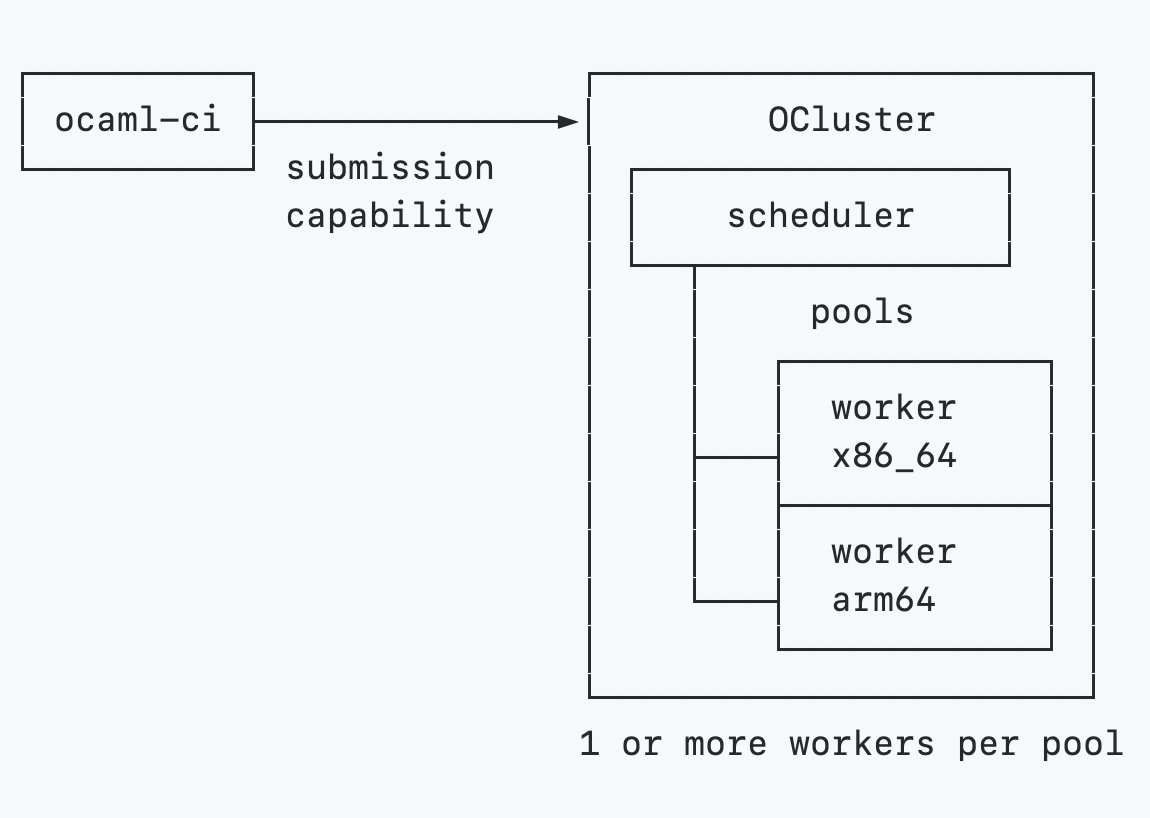
\includegraphics[width=\linewidth]{ocluster-arch.png}
  \caption{ocluster architecture}
  \label{fig:arch1}
\end{figure}

Workers are responsible for providing a sandboxed execution using the implementation available on that plaform, and providing a store for caching build steps to avoid repeating the execution. For each platform we want to support, we need to provide a solution for the sandbox and store.

\begin{figure}
  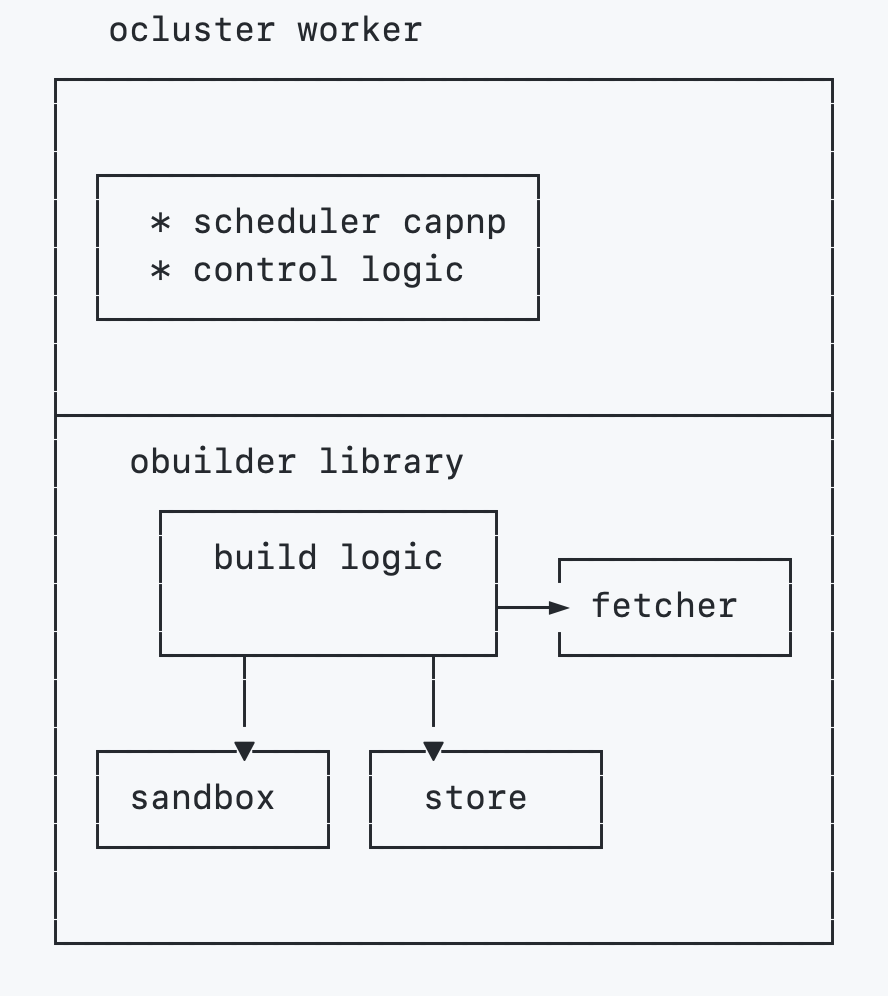
\includegraphics[width=\linewidth]{obuilder-arch.png}
  \caption{obuilder architecture}
  \label{fig:arch1}
\end{figure}

\section{Implementation on Linux}

OBuilder on Linux grew out of the need to replace BuildKit, the underlying technology used for docker build on Linux. On Linux the sandboxing is provided by runc and native containerisation. `runc` is a CLI tool for spawning and running containers on Linux according to the OCI specification. The mechanisms used are based on Linux's native namespaces and cgroups functionality, as used by BuildKit. The key feature of namespaces is that they isolate processes from each other, while cgroups control how much of a given key resource a process has access to. 

For the store Linux provides two filesystems with efficient snapshot support, Btrfs and ZFS. The Btrfs store uses Btrfs subvolumes to snapshot and restore filesystem state. While under ZFS the native snapshotting support is used. The current ocluster provided for systems like ocaml-ci and opam-ci uses Linux with Btrfs.

\section{Implementation on macOS}
Supporting OBuilder on macOS required overcoming the major shortcoming that macOS does not provide a native containerisation solution. You cannot carve up macOS using namespaces or limit resource access using cgroups, like you would with Linux. However, you can have multiple users on a single machine, each with their own home directory and ability to execute commands. This user isolation approach forms the basis of the sandboxing on macOS. Looking at our restricted use case of building OCaml packages we needed to solve two extra problems, how to isolate opam installations and second how to sandbox native dependencies on macOS.

Opam supports having multiple opam roots on a system typically in the home directory of the user \texttt{\textasciitilde/.opam} , which complements the user isolation approach. You can run something like \texttt{sudo -u macos-builder-705 -i /bin/bash -c 'opam install irmin'} and it will use macos-builder-705’s home directory to build irmin. This provides a level of isolation similar to runc on Linux.

Homebrew, a macOS system package manager, used by opam for installing native libraries, is not so flexible. It wants to be installed globally at a fixed location in \texttt{/usr/local}. The official documentation saying you could install it elsewhere but \emph{"Pick another prefix at your peril!"}\footnote{https://docs.brew.sh/Installation\#untar-anywhere}. To fully sandbox a build you need to containerise homebrew. The solution chosen uses FUSE (file system in user space) to setup a faked system installation of homebrew packages per user, which then gets used by Opam via depext. The proposed solution is to mount a FUSE (filesystem in userspace) filesystem onto /usr/local which intercepts calls and redirects them based on who the calling user is. Before the build an empty homebrew directory is provided, then during the build opam installs native packages and afterwards the modified contents are discarded, with the next build starting back at the beginning with an empty homebrew install.

Providing the snapshotting store is a challenge on macOS as the native macOS file system APFS doesn’t provide the snapshotting control required for OBuilder. There is a port of ZFS that provided some initial promise but after many hours were lost debugging many small bugs in ZFS, we opted for a portable and reliable solution using rsync. The obvious trade-off being it was slower and memory inefficient using rsync as the store backend. Rsync is used to snapshot the home directory of the user while performing a build and to restore it from the stored snapshots.

Equipped with both rsync, user isolation and a sense that we needed to perform some file system indirection, a macOS implementation of OBuilder emerged. This implementation is currently providing builds on the opam repository, checking packages before they are published to opam.

\section{Implementation on Windows}

The Windows support for OBuilder could have used a similar approach to macOS, using user isolation and intelligent file syncing to provide a sandbox and store implementation respectively. However, Windows does have native containers and it does have the tools for assembling a snapshotting filesystem. The choice was made not to use these, why? Direct access to these technologies is considerably harder and less stable than their Linux counterparts, no bindings exist for the Windows native containers and the API provided is not official or stable. Building them is a large undertaking however we plan to revisit them in future. So we turned to using Docker on Windows, which had the advantage of a more stable base with many active users and the interfacing to native Windows containers is handled for us. 

Under Windows the sandbox is provided by a Windows container with opam and ocaml already installed, which is started and then used to execute the build spec inside. By using a container we can address a shortcoming of Docker for Windows which prevents docker build from using more than 2CPU on the host \cite{2CPUWindows18}. Two modes of sandboxing are available: either full virtualisation through the Hyper-V hypervisor, or process-level isolation using Windows Native Containers. We use VMs by default, with the cost of longer boot and execution time, but hopefully better security and stability.

The store implementation on Windows uses Docker images, where a base Docker image is taken for the base of the build step, then the command runs in a Docker container, and if the build step succeeds, the resulting base image gets tagged and committed to a new image used as the base for the next build step. Each Docker image is tagged with the id of the build step so that they can be reused.

While using Docker directly might seem straight-forward, implementing it required fixing OCaml’s Unix library and LWT's Windows support, as well as some creative use of Docker. This same architecture allows for running OBuilder using docker on Linux, at the cost of some performance and bringing us full circle. Back running builds using docker but this time inside a docker container rather than using docker build directly.

\section{Conclusion}

We have presented OBuilder, a light weight sandboxing solution, used to provide a homogeneous builds for OCaml with OCaml. Our work has built on the existing Linux containerisation implementation by extending it to work with macOS and Windows. The macOS implementation relied on user isolation, FUSE and rsync to provide a sandbox environment and store. While Windows support re-used the existing Docker for Windows capabilities in an interesting way to provide those capabilties.

\section{Future Work}

The OBuilder support described for macOS/x86 workers is already available in OCluster and is being used to check opam repository PRs. After that we want to address the 1 user per macOS worker limitation and to scale out the underlying hardware for macOS/x86 to support runing ocaml-ci.

For the Windows workers we have tested deployments and succesfully run builds on them. With the next step being integrating them into the opam repository PR checks, and after that adding ocaml-ci support. As a consequence of this work, when packages are released on opam, their support for Windows and macOS is demonstrated as they are built.

On Windows there is an experimental container orchestration tool hcsrun that we would like to try, as well as snapshotting filesystem support Btrfs for Windows \cite{BtrfsWindows16}. These native solutions promise better resource usage of the underlying hardware, translating into more capacity for running builds.

Supporting the BSDs is another focus, with the preliminary support for Docker on FreeBSD we have experimented with using runj \cite{runj21}, (a new experimental, proof-of-concept OCI-compatible runtime for FreeBSD jails) to add FreeBSD support and reusing ZFS from Linux support for snapshotting the file system. 

\bibliographystyle{ACM-Reference-Format}
\bibliography{refs}

\end{document}
%%